\documentclass[12pt]{article}
\usepackage{setspace, graphicx, fullpage, amssymb, amsmath, epsfig, natbib, array, multirow, hyperref}
\usepackage{amsfonts, bm} 
\usepackage{dcolumn}
\usepackage{subfigure, float} 
\usepackage[margin=1.25in]{geometry} 
\usepackage{verbatim}
\usepackage{url}
\usepackage{enumerate}
\newcolumntype{d}[1]{D{.}{.}{#1}} 

\begin{document}
	
	\begin{center}
		Update: 30 December 2016
	\end{center}

In preparation for our meeting, I present you with what I've found over the past week. Having transformed the ideology/extremism variables to match standard usage in the House and Senate I find that we still have the same problems in the Senate. Reverting entirely to the methods we previously used to construct the covariates found in \verb|senator_year_data|\footnote{With a few slight corrections. I had forgotten to uncomment the part of the script that corrected Sen. D'Amato's name and reviewing the data we got from Wiseman revealed that we had previously failed to note 4 female Senators.}. The sorting method that relies only on the switch to \verb|emIRT()| in the Senate gives us variables in line with what we would expect, however, our other two sets still give us problems. Specifically, it appears that the explanatory power of ideological extremism is being taken by the presidential vote share variable for some reason in the hybrid and flip flop reassignment based analyses. The regression tables are included below.

I checked to make sure there were not large differences between the variables produced by the different sorting methods by checking the \verb|emIRT()| only model against the hybrid model, focusing on Democrats (though I also looked at the whole dataset). The results are found in the figure below. It does not appear that there are differences beyond what we would anticipate. Nor are there differences between the covariates in the datasets. I propose that we spend some amount of time either figuring out what is likely to be going on or discussing what tools I could employ in order to determine what is going on in the coming week.

\begin{table}
	\begin{center}
    	\caption{emIRT Only, Party Analysis}
		\begin{tabular}{l c c }
			\hline
			& Democrats & Republicans \\
			\hline
			ideological\_extremism   & $3.720^{***}$  & $7.028^{***}$  \\
			& $(0.415)$      & $(0.359)$      \\
			chair                    & $1.755^{**}$   & $4.056^{***}$  \\
			& $(0.538)$      & $(0.697)$      \\
			responsiveness\_noncalls & $0.859^{***}$  & $0.897^{***}$  \\
			& $(0.035)$      & $(0.035)$      \\
			vote\_share              & $-4.109$       & $14.207^{***}$ \\
			& $(2.172)$      & $(2.785)$      \\
			\textbf{pres\_vote\_share}        & $16.868^{***}$ & $-9.455^{**}$  \\
			& $(2.432)$      & $(3.022)$      \\
			power\_committee         & $-0.049$       & $0.440$        \\
			& $(0.773)$      & $(0.923)$      \\
			south13                  & $-1.056$       & $0.413$        \\
			& $(0.554)$      & $(0.570)$      \\
			female                   & $1.892^{**}$   & $0.092$        \\
			& $(0.698)$      & $(1.084)$      \\
			afam                     & $-0.236$       & $-5.485$       \\
			& $(2.715)$      & $(4.133)$      \\
			latino                   & $2.360$        & $5.875^{*}$    \\
			& $(2.276)$      & $(2.670)$      \\
			up\_for\_reelection      & $-0.483$       & $-1.202^{*}$   \\
			& $(0.410)$      & $(0.510)$      \\
			seniority                & $-0.053$       & $0.094$        \\
			& $(0.058)$      & $(0.079)$      \\
			freshman                 & $-1.146^{*}$   & $2.661^{***}$  \\
			& $(0.576)$      & $(0.752)$      \\
			retiree                  & $5.021$        & $1.067$        \\
			& $(3.037)$      & $(2.874)$      \\
			best\_committee          & $-0.060$       & $-0.087$       \\
			& $(0.127)$      & $(0.161)$      \\
			leader                   & $2.143^{*}$    & $2.129$        \\
			& $(1.008)$      & $(1.182)$      \\
			(Intercept)              & $3.637$        & $-0.805$       \\
			& $(3.396)$      & $(3.461)$      \\
			\hline
			R$^2$                    & 0.696          & 0.668          \\
			Adj. R$^2$               & 0.691          & 0.662          \\
			Num. obs.                & 988            & 901            \\
			RMSE                     & 5.956          & 6.959          \\
			\hline
			\multicolumn{3}{l}{\scriptsize{$^{***}p<0.001$, $^{**}p<0.01$, $^*p<0.05$}}
		\end{tabular}
	\end{center}
\end{table}

\begin{table}
	\begin{center}
	\caption{emIRT Only, Majority Analysis}
		\begin{tabular}{l c c }
			\hline
			& Majority & Minority \\
			\hline
			ideological\_extremism   & $4.364^{***}$  & $7.128^{***}$ \\
			& $(0.326)$      & $(0.383)$     \\
			chair                    & $-0.026$       & $5.038^{***}$ \\
			& $(0.551)$      & $(1.249)$     \\
			responsiveness\_noncalls & $0.847^{***}$  & $0.889^{***}$ \\
			& $(0.031)$      & $(0.036)$     \\
			vote\_share              & $-2.219$       & $7.029^{**}$  \\
			& $(2.231)$      & $(2.659)$     \\
			pres\_vote\_share        & $12.588^{***}$ & $3.602$       \\
			& $(2.028)$      & $(2.969)$     \\
			power\_committee         & $0.419$        & $-0.872$      \\
			& $(0.748)$      & $(0.978)$     \\
			south13                  & $0.228$        & $0.549$       \\
			& $(0.459)$      & $(0.554)$     \\
			female                   & $0.997$        & $2.412^{*}$   \\
			& $(0.769)$      & $(0.974)$     \\
			afam                     & $2.811$        & $-3.435$      \\
			& $(4.008)$      & $(3.031)$     \\
			latino                   & $0.749$        & $8.200^{**}$  \\
			& $(2.316)$      & $(2.628)$     \\
			up\_for\_reelection      & $-0.782$       & $-0.812$      \\
			& $(0.412)$      & $(0.526)$     \\
			seniority                & $0.108$        & $0.046$       \\
			& $(0.067)$      & $(0.070)$     \\
			freshman                 & $-0.517$       & $0.985$       \\
			& $(0.595)$      & $(0.750)$     \\
			retiree                  & $0.933$        & $4.791$       \\
			& $(2.569)$      & $(3.669)$     \\
			best\_committee          & $0.044$        & $-0.276$      \\
			& $(0.125)$      & $(0.166)$     \\
			leader                   & $0.978$        & $2.783^{*}$   \\
			& $(1.043)$      & $(1.188)$     \\
			(Intercept)              & $5.079$        & $-2.350$      \\
			& $(3.216)$      & $(3.665)$     \\
			\hline
			R$^2$                    & 0.704          & 0.654         \\
			Adj. R$^2$               & 0.698          & 0.647         \\
			Num. obs.                & 886            & 907           \\
			RMSE                     & 5.612          & 7.295         \\
			\hline
			\multicolumn{3}{l}{\scriptsize{$^{***}p<0.001$, $^{**}p<0.01$, $^*p<0.05$}}
		\end{tabular}
	\end{center}
\end{table}

\begin{table}
	\begin{center}
		\caption{Random Reassignment of Flip Flop Votes, Party Analysis}
		\begin{tabular}{l c c }
			\hline
			& Democrats & Republicans \\
			\hline
			ideological\_extremism   & $-3.770^{***}$ & $2.898^{***}$  \\
			& $(0.741)$      & $(0.571)$      \\
			chair                    & $-1.771^{**}$  & $-2.589^{***}$ \\
			& $(0.661)$      & $(0.751)$      \\
			responsiveness\_noncalls & $0.831^{***}$  & $0.891^{***}$  \\
			& $(0.036)$      & $(0.032)$      \\
			vote\_share              & $-4.670$       & $4.824$        \\
			& $(2.624)$      & $(2.974)$      \\
			\textbf{pres\_vote\_share}        & $30.274^{***}$ & $-4.604$       \\
			& $(2.946)$      & $(3.193)$      \\
			power\_committee         & $0.014$        & $1.386$        \\
			& $(0.934)$      & $(0.975)$      \\
			south13                  & $-3.562^{***}$ & $-0.284$       \\
			& $(0.654)$      & $(0.596)$      \\
			female                   & $-0.366$       & $0.912$        \\
			& $(0.845)$      & $(1.140)$      \\
			afam                     & $4.289$        & $-7.377$       \\
			& $(3.277)$      & $(4.361)$      \\
			latino                   & $-1.296$       & $-7.184^{*}$   \\
			& $(2.755)$      & $(2.825)$      \\
			up\_for\_reelection      & $-0.521$       & $-0.054$       \\
			& $(0.495)$      & $(0.541)$      \\
			seniority                & $-0.029$       & $0.149$        \\
			& $(0.070)$      & $(0.083)$      \\
			freshman                 & $-0.766$       & $0.587$        \\
			& $(0.699)$      & $(0.803)$      \\
			retiree                  & $2.853$        & $2.125$        \\
			& $(3.650)$      & $(3.042)$      \\
			best\_committee          & $-0.131$       & $0.243$        \\
			& $(0.154)$      & $(0.169)$      \\
			leader                   & $-0.788$       & $0.434$        \\
			& $(1.219)$      & $(1.255)$      \\
			(Intercept)              & $6.468$        & $4.838$        \\
			& $(3.427)$      & $(3.190)$      \\
			\hline
			R$^2$                    & 0.630          & 0.663          \\
			Adj. R$^2$               & 0.624          & 0.657          \\
			Num. obs.                & 987            & 901            \\
			RMSE                     & 7.193          & 7.362          \\
			\hline
			\multicolumn{3}{l}{\scriptsize{$^{***}p<0.001$, $^{**}p<0.01$, $^*p<0.05$}}
		\end{tabular}
	\end{center}
\end{table}

\begin{table}
	\begin{center}
	\caption{Random Reassignment of Flip Flop Votes, Majority Analysis}
		\begin{tabular}{l c c }
			\hline
			& Majority & Minority \\
			\hline
			ideological\_extremism   & $-1.106$       & $1.692^{**}$   \\
			& $(0.714)$      & $(0.597)$      \\
			chair                    & $-1.837^{*}$   & $-3.319^{**}$  \\
			& $(0.731)$      & $(1.281)$      \\
			responsiveness\_noncalls & $0.866^{***}$  & $0.894^{***}$  \\
			& $(0.038)$      & $(0.032)$      \\
			vote\_share              & $5.906^{*}$    & $-4.279$       \\
			& $(2.979)$      & $(2.690)$      \\
			\textbf{pres\_vote\_share}        & $13.942^{***}$ & $16.404^{***}$ \\
			& $(2.751)$      & $(2.932)$      \\
			power\_committee         & $1.546$        & $-0.617$       \\
			& $(0.994)$      & $(0.992)$      \\
			south13                  & $-0.126$       & $-1.600^{**}$  \\
			& $(0.610)$      & $(0.564)$      \\
			female                   & $0.720$        & $1.462$        \\
			& $(1.019)$      & $(0.985)$      \\
			afam                     & $0.467$        & $-1.176$       \\
			& $(5.313)$      & $(3.076)$      \\
			latino                   & $0.429$        & $-5.746^{*}$   \\
			& $(3.073)$      & $(2.673)$      \\
			up\_for\_reelection      & $0.159$        & $-0.898$       \\
			& $(0.547)$      & $(0.534)$      \\
			seniority                & $0.097$        & $0.098$        \\
			& $(0.091)$      & $(0.071)$      \\
			freshman                 & $0.873$        & $0.596$        \\
			& $(0.791)$      & $(0.763)$      \\
			retiree                  & $-1.177$       & $8.162^{*}$    \\
			& $(3.400)$      & $(3.724)$      \\
			best\_committee          & $0.212$        & $-0.193$       \\
			& $(0.166)$      & $(0.169)$      \\
			leader                   & $0.634$        & $-1.306$       \\
			& $(1.384)$      & $(1.210)$      \\
			(Intercept)              & $-1.659$       & $3.084$        \\
			& $(3.789)$      & $(3.147)$      \\
			\hline
			R$^2$                    & 0.576          & 0.670          \\
			Adj. R$^2$               & 0.569          & 0.664          \\
			Num. obs.                & 885            & 907            \\
			RMSE                     & 7.437          & 7.406          \\
			\hline
			\multicolumn{3}{l}{\scriptsize{$^{***}p<0.001$, $^{**}p<0.01$, $^*p<0.05$}}
		\end{tabular}
	\end{center}
\end{table}

\begin{table}
	\begin{center}
		\caption{Hybrid Model, Party Analysis}
		\begin{tabular}{l c c }
			\hline
			& Democrats & Republicans \\
			\hline
			ideological\_extremism   & $-3.793^{***}$ & $3.037^{***}$  \\
			& $(0.743)$      & $(0.590)$      \\
			chair                    & $-1.747^{**}$  & $-2.995^{***}$ \\
			& $(0.663)$      & $(0.773)$      \\
			responsiveness\_noncalls & $0.845^{***}$  & $0.890^{***}$  \\
			& $(0.037)$      & $(0.033)$      \\
			vote\_share              & $-4.258$       & $6.099^{*}$    \\
			& $(2.633)$      & $(3.062)$      \\
			\textbf{pres\_vote\_share}        & $30.329^{***}$ & $-6.433$       \\
			& $(2.954)$      & $(3.289)$      \\
			power\_committee         & $-0.022$       & $1.601$        \\
			& $(0.937)$      & $(1.004)$      \\
			south13                  & $-3.569^{***}$ & $-0.215$       \\
			& $(0.656)$      & $(0.613)$      \\
			female                   & $-0.479$       & $1.485$        \\
			& $(0.848)$      & $(1.174)$      \\
			afam                     & $4.247$        & $-7.187$       \\
			& $(3.287)$      & $(4.490)$      \\
			latino                   & $-1.077$       & $-5.861^{*}$   \\
			& $(2.765)$      & $(2.908)$      \\
			up\_for\_reelection      & $-0.510$       & $-0.041$       \\
			& $(0.497)$      & $(0.557)$      \\
			seniority                & $-0.038$       & $0.200^{*}$    \\
			& $(0.070)$      & $(0.086)$      \\
			freshman                 & $-0.752$       & $0.888$        \\
			& $(0.701)$      & $(0.827)$      \\
			retiree                  & $3.116$        & $1.573$        \\
			& $(3.662)$      & $(3.132)$      \\
			best\_committee          & $-0.136$       & $0.244$        \\
			& $(0.154)$      & $(0.174)$      \\
			leader                   & $-0.808$       & $0.381$        \\
			& $(1.223)$      & $(1.292)$      \\
			(Intercept)              & $5.022$        & $4.618$        \\
			& $(3.441)$      & $(3.289)$      \\
			\hline
			R$^2$                    & 0.634          & 0.650          \\
			Adj. R$^2$               & 0.628          & 0.644          \\
			Num. obs.                & 987            & 901            \\
			RMSE                     & 7.217          & 7.580          \\
			\hline
			\multicolumn{3}{l}{\scriptsize{$^{***}p<0.001$, $^{**}p<0.01$, $^*p<0.05$}}
		\end{tabular}
	\end{center}
\end{table}

\begin{table}
	\begin{center}
		\caption{Hybrid Model, Majority Analysis}
		\begin{tabular}{l c c }
			\hline
			& Majority & Minority \\
			\hline
			ideological\_extremism   & $-1.122$       & $1.717^{**}$   \\
			& $(0.728)$      & $(0.611)$      \\
			chair                    & $-1.931^{**}$  & $-3.503^{**}$  \\
			& $(0.741)$      & $(1.309)$      \\
			responsiveness\_noncalls & $0.878^{***}$  & $0.900^{***}$  \\
			& $(0.039)$      & $(0.033)$      \\
			vote\_share              & $6.804^{*}$    & $-3.889$       \\
			& $(3.023)$      & $(2.750)$      \\
			\textbf{pres\_vote\_share}        & $12.512^{***}$ & $17.201^{***}$ \\
			& $(2.791)$      & $(2.995)$      \\
			power\_committee         & $1.654$        & $-0.584$       \\
			& $(1.008)$      & $(1.014)$      \\
			south13                  & $-0.109$       & $-1.643^{**}$  \\
			& $(0.618)$      & $(0.577)$      \\
			female                   & $0.826$        & $1.753$        \\
			& $(1.034)$      & $(1.007)$      \\
			afam                     & $0.281$        & $-1.071$       \\
			& $(5.387)$      & $(3.144)$      \\
			latino                   & $0.777$        & $-4.477$       \\
			& $(3.117)$      & $(2.732)$      \\
			up\_for\_reelection      & $0.123$        & $-0.811$       \\
			& $(0.555)$      & $(0.546)$      \\
			seniority                & $0.121$        & $0.104$        \\
			& $(0.092)$      & $(0.073)$      \\
			freshman                 & $1.181$        & $0.604$        \\
			& $(0.802)$      & $(0.780)$      \\
			retiree                  & $-1.200$       & $8.100^{*}$    \\
			& $(3.448)$      & $(3.806)$      \\
			best\_committee          & $0.214$        & $-0.212$       \\
			& $(0.169)$      & $(0.173)$      \\
			leader                   & $0.525$        & $-1.218$       \\
			& $(1.403)$      & $(1.237)$      \\
			(Intercept)              & $-2.928$       & $1.912$        \\
			& $(3.853)$      & $(3.219)$      \\
			\hline
			R$^2$                    & 0.572          & 0.663          \\
			Adj. R$^2$               & 0.564          & 0.657          \\
			Num. obs.                & 885            & 907            \\
			RMSE                     & 7.542          & 7.571          \\
			\hline
			\multicolumn{3}{l}{\scriptsize{$^{***}p<0.001$, $^{**}p<0.01$, $^*p<0.05$}}
		\end{tabular}
	\end{center}
\end{table}

\begin{figure}[h]
	\caption{Comparisons of Senate Variables for Democrats}
	\centering
	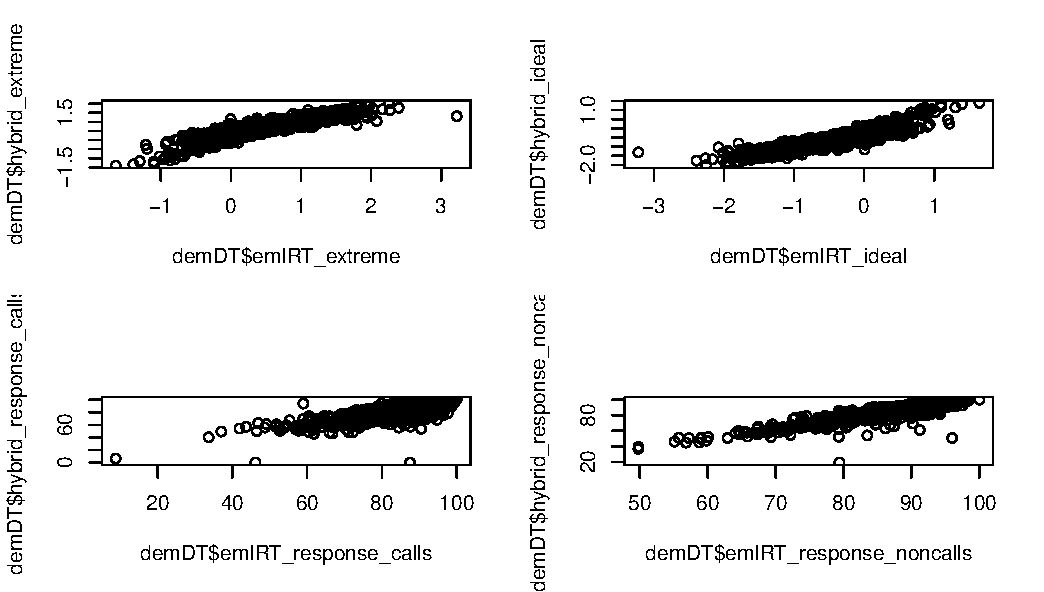
\includegraphics[]{C:/Users/Ethan/Documents/GitHub/partycalls/plots/check_democrat_variables.pdf}
	
\end{figure}


















\end{document}